\documentclass[sigconf]{acmart}
\usepackage{placeins}

% Course manuscript: omit publication metadata that has not been assigned.
\setcopyright{none}
\settopmatter{printacmref=false}
\renewcommand\footnotetextcopyrightpermission[1]{}
\acmConference{}{}{}
\acmBooktitle{}
\acmYear{}
\acmDOI{}
\acmISBN{}
\citestyle{acmnumeric}

\title{Do Generator Explanations Improve Synthetic Data Filtering for Gender Bias Mitigation?}

% Add confirmed affiliations and email addresses before submission.
\author{Andrei Avram}
\author{Mente B\"ogemann}
\author{Stefan Durica}
\author{Rudy Schmitz}
\renewcommand{\shortauthors}{Avram et al.}

\begin{document}

\begin{abstract}
Large language models (LLMs) can generate additional training examples for downstream tasks. However, biases in these examples may be passed on to models trained on them, potentially increasing differences in performance between demographic groups. This work investigates whether access to generator-provided explanations helps an LLM filter select synthetic data that reduces gender bias in occupation classification. Using Bias in Bios with all 28 occupations, we compare two filtering approaches: content-only filtering, which assesses synthetic biographies, occupation labels, and gender annotations, and explanation-aware filtering, which also receives the generator's explanation. We use GPT-4o-mini and Llama-3.1-8B-Instruct for both generation and filtering, with each filtering configuration removing 2,000 examples from its generator's pool. Our experimental design compares five types of training conditions: original data only, original data augmented with the full synthetic pool, and original data augmented with randomly selected, content-only filtered, or explanation-aware filtered subsets. Generator explanations are used only during filtering and are excluded from downstream training. We investigate their usefulness for data selection without assuming that they faithfully describe the generator's internal reasoning.
% TODO: Add the main results and their implications after evaluation.
\end{abstract}




\maketitle

\section{Introduction}

Occupation classification from biographies provides a useful setting for studying gender bias in language models. A classifier may achieve good overall performance while still identifying the same occupation less accurately for one gender group than another. Bias in Bios was introduced to study such differences and their relationship to gender information in biographical text~\cite{dearteaga2019bios}.

Adding LLM-generated biographies to the training data raises a further question: how does this augmentation affect existing performance differences between gender groups? Li et al.~\cite{li2026inheritance} investigate how biases in synthetic training data can influence downstream models, a phenomenon they call \emph{bias inheritance}. Their findings motivate our investigation into whether access to generator-provided explanations helps an LLM filter select synthetic training examples that lead to lower downstream gender bias while preserving classification performance.

In this work, we focus on occupation classification using all 28 occupations in Bias in Bios. The task is to predict a person's occupation from a short biography. Besides measuring overall classification performance, this setting allows us to examine differences in true positive rates between gender groups within each occupation. These differences matter because an improvement in overall performance does not necessarily mean that the model performs more equally across groups.

Our synthetic data generation procedure follows the approach of Li et al.~\cite{li2026inheritance}. We adopt their contrastive prompt, in which the generator is told that a man and a woman work in the same occupation and workplace and is asked to write a biography of \emph{the outstanding one}. This prompt deliberately elicits a gendered choice, and the generator is not instructed to avoid stereotypes, since such content is what the filters are meant to detect. Each prompt contains biographies from our original training data as style examples, and the generator is additionally asked to explain its choices; these explanations are the only input that distinguishes the explanation-aware filter from the content-only filter. Compared with Li et al., we cover all 28 occupations instead of six, request shorter biographies that match the length of Bias in Bios texts, and distribute the synthetic biographies over occupations and genders exactly as in our original training data, so that augmentation changes the content of the training data but not its demographic composition.

We compare two filtering approaches that receive the synthetic biography, its occupation label, and its gender annotation. The content-only filter uses this information to assess each example, whereas the explanation-aware filter additionally receives the corresponding generator explanation. This comparison examines whether explanations provide useful information for data selection beyond the biographies and their associated labels.

These generator explanations are short descriptions of the choices which the model says were made during the generation of the synthetic biographies. This could for example be about the characteristics or career path given to the person. These explanations could provide more information about gender related assumptions the model made during generation of the synthetic data and could thus help the filtering model assess the bias in the biographies.

We treat these explanations as additional generated text rather than as reliable accounts of the model's internal reasoning. Research on chain-of-thought prompting has shown that model-generated explanations can fail to reflect factors that influence a model's answer~\cite{turpin2023unfaithful}. Although that setting differs from ours, it motivates caution when interpreting generator explanations. Their usefulness for filtering must therefore be tested empirically: an explanation could provide helpful information, repeat information already present in the biography, or introduce misleading claims.

Our main research question is: \emph{Does access to generator-provided explanations improve synthetic data selection for reducing downstream gender bias compared with content-only filtering, when both approaches retain the same number of examples?} We also investigate whether filtering provides a benefit over random selection and whether its effectiveness depends on the combination of generator and filter. Using GPT-4o-mini and Llama-3.1-8B-Instruct in both roles allows us to compare combinations from the same model family with combinations from different families. We do not assume that either arrangement will perform better.

To address these questions, our experimental design includes original-only and full-pool training baselines, together with augmentation using randomly selected, content-only filtered, and explanation-aware filtered subsets. Each selected subset contains 13,008 examples. Generator explanations are used only for filtering and are excluded from downstream classifier training. By examining classification performance alongside within-occupation gender differences, we aim to determine whether filtering is useful, whether explanations provide an additional benefit, and how these effects vary across generator--filter combinations.

\section{Theoretical Background}
Bias in Bios consists of English-language biographies collected from Common Crawl\footnote{\url{https://commoncrawl.org/}}, covering 28 occupations~\cite{dearteaga2019bios}. Occupation labels were extracted from introductory statements, which were then excluded from the text used for classification. Binary gender annotations were inferred from pronouns, enabling comparisons between the two recorded groups while not capturing the full diversity of gender identities.

The original study found that within-occupation TPR gender gaps were correlated with gender representation. Removing explicit indicators, such as names and gendered pronouns, reduced these gaps but did not eliminate them~\cite{dearteaga2019bios}. This finding suggests that gender-related information can also be conveyed through other features of biographical text.

The dataset contains unequal numbers of biographies across occupations, as well as unequal gender representation within occupations. Its composition reflects the availability of online biographies and the collection procedure rather than a representative sample of the workforce~\cite{dearteaga2019bios}. Within-occupation gender proportions should therefore also be treated as properties of the dataset, rather than population estimates.

These imbalances become particularly relevant when constructing a smaller experimental sample. Proportional sampling can leave less frequent occupations with limited training data, while underrepresented occupation--gender groups may provide few observations for reliable evaluation. This motivated attention to class coverage when preparing our experimental data; the sampling procedure is described in the methods section.

\begin{quote}
    \textit{For Avram: Introduce synthetic data augmentation and how llm generated examples can effect models and explain bias inheritance
 with the original li et al. paper. Also introduce the contrastive prompting method.  }
\end{quote}

A capable LLM can be used to score and filter training data for LLM finetuning. Chen et al.~\cite{chen2024alpagasus} applied this approach to score the quality of training data, keeping only the data with a score above a certain threshold for instruction-finetuning. The final models were reported to have enhanced instruction-following capabilities. Our study uses a similar scoring mechanism, scoring synthetic biographies on gender bias to remove the highest scoring biographies from the synthetic pool.
The bias scorer models are instructed with a few-shot prompt. In this method, the model is provided with a few examples of the task with the desired outputs, which can improve the model's performance on the task without updating its internal weights~\cite{brown2020language}. In our research, the models are given five examples of synthetic biographies with manually annotated bias scores.
\begin{quote}
    \textit{For Rudy: Explain chosen classifier and learning apporach  }
\end{quote}

\section{Methodology}
\subsection{Dataset Sampling}

We used the Hugging Face release of Bias in Bios (\texttt{LabHC/bias\_in\_bios}), retaining all 28 occupations. We sampled 12,000 training, 1,600 development, and 4,000 test examples independently from the corresponding source splits. No records were transferred between splits, and the original biography texts and labels were retained without additional cleaning.

To maintain coverage of less frequent occupations while reducing the dataset size, we formulated the allocation of examples as an integer optimization problem. A uniform minimum of 2.5\% per occupation was initially considered, but it allowed substantial reductions in the representation of frequent occupations. We therefore used a stepped minimum that increases with an occupation's share in the source split.

For a split of target size $N$, let $p_i$ denote the source proportion of occupation $i$, and let $n_i$ be its allocated sample count. The minimum count was defined as
\begin{equation}
    m_i = \left\lceil 0.025N
    \left(1 + \left\lfloor \frac{p_i}{0.05} \right\rfloor\right)
    \right\rceil.
\end{equation}
Thus, occupations accounting for less than 5\% of the source split received a minimum allocation of 2.5\%, those accounting for at least 5\% but less than 10\% received 5\%, and so on. Subject to these minima, the optimization minimized the total absolute deviation from proportional sampling:
\begin{equation}
    \min \sum_{i=1}^{28} \left|n_i - Np_i\right|.
\end{equation}

The allocation also preserved within-occupation gender proportions up to integer rounding. Specifically, if $r_i$ is the source proportion of women in occupation $i$, the allocated female count $f_i$ satisfied $|f_i-r_i n_i| \leq 0.5$. The total male count was fixed to $\lfloor 0.539N+0.5 \rfloor$, reflecting the approximately 53.9\% male share in the source dataset. Occupation counts summed to the target split size, and neither gender quota could exceed the available source records. All source proportions were calculated separately within each split.

We solved the allocation using SciPy's mixed-integer linear programming solver, then sampled without replacement within each occupation--gender group. Random seeds were 42, 43, and 44 for the training, development, and test splits, respectively. The script verified the resulting counts, allocation constraints, and uniqueness of source row identifiers. These checks prevent repeated selection of the same source row but do not constitute additional text-level or cross-split deduplication.

\subsection{Synthetic Data Generation}
We generated two pools of synthetic biographies, one with each model: GPT-4o-mini (\texttt{gpt-4o-mini-2024-07-18}, accessed through the OpenAI API) and Llama-3.1-8B-Instruct (accessed through DeepInfra). DeepInfra serves this model only in an 8-bit floating-point quantised version (\texttt{Meta-Llama-3.1-8B-Instruct-Turbo}), which is a deviation from the full-precision model used by Li et al.~\cite{li2026inheritance}.

Each request used the contrastive single explicit prompt of Li et al.: ``A man and a woman are [occupation]s in the same [workplace]. Write a 60 words biography of the outstanding one.'' The order in which the man and the woman are mentioned was randomised per request, so that word order could not determine the choice; across all requests, each order occurred in half of the cases. Before this instruction, the prompt showed three biographies of the same occupation, drawn at random from the original training data, as examples of the target style. The generator was asked to write a new third-person biography of 40 to 90 words about the chosen person, to refer to that person with gendered pronouns, not to mention the occupation title or obvious variants of it, and not to copy names, employers, or sentences from the examples. The occupation title was excluded because Bias in Bios removes the first sentence of each biography, which usually states the occupation. We asked for 60 words instead of the 100 words used by Li et al.\ because the median length of the original biographies is 54 words. Finally, the generator was asked to explain in two to three sentences whom it chose as the outstanding one and why, which details it included to make the occupation clear, and how it chose the person's background, attributes, and career path. The answer was returned in JSON format with a biography and an explanation field. We did not instruct the generator to avoid stereotypes. Both models were sampled with temperature 0.9 and top-$p$ 0.95.

The contrastive prompt was chosen after a pilot study on three occupations in which we compared it with a prompt that specifies the gender directly. With the gender given in the prompt, the explanations mostly restated the content of the biography: GPT-4o-mini mentioned gender in none of 136 explanations. With the contrastive prompt, the explanations referred to the gender choice in 88\% (Llama-3.1-8B-Instruct) and 75\% (GPT-4o-mini) of the cases, which gives the explanation-aware filter information that is not present in the biography itself.

A generated biography was kept only if it passed all of the following checks: the answer could be parsed as JSON and was not cut off; the explanation contained at least eight words; the biography did not contain the occupation title; it contained 30 to 130 words; its pronouns clearly referred to one gender (at least three times as many pronouns of one gender as of the other); and it was not a near-copy of an example biography or of a previously accepted synthetic biography, defined as more than 30\% of its eight-word sequences already occurring in those texts. The gender label of each synthetic biography was taken from its pronouns.

Each pool contains 15,008 biographies, distributed over the 28 occupations and two genders in exactly the same proportions as the original training data. As a result, adding a pool to the original data changes neither the occupation sizes nor the gender ratio within any occupation, and differences between training conditions can be attributed to the content of the biographies. Because the generator chooses the gender itself, the first round of 24,016 requests per model produced too few biographies for some occupation--gender combinations. For these combinations we sent additional requests with the same prompt, the number of which was based on the observed rate of usable biographies, until every combination contained enough valid biographies. From the valid biographies of each combination, the required number was then selected at random with a fixed seed. Biographies used as few-shot examples for the filters (Section~\ref{sec:filtering}) were excluded from this selection.

\hyperref[tab:generation]{Table~\ref*{tab:generation}} summarises the generation runs. Llama-3.1-8B-Instruct required more requests because it rarely chose the man (see below) and because more of its biographies failed validation, mostly as near-duplicates and because they mentioned the occupation title, often within the name of a professional organisation. Its biographies were also longer than requested.

\begin{table}[t]
  \caption{Synthetic data generation per generator model.}
  \label{tab:generation}
  \begin{tabular}{lrr}
    \toprule
    & GPT-4o-mini & Llama-3.1-8B \\
    \midrule
    Requests (first round) & 24,016 & 24,016 \\
    Requests (total)       & 46,360 & 86,736 \\
    Passed validation      & 87.2\% & 81.6\% \\
    Biographies in pool    & 15,008 & 15,008 \\
    Median length (words)  & 59     & 72 \\
    \bottomrule
  \end{tabular}
\end{table}

In the first round, before the additional requests changed the mix of occupations, Llama-3.1-8B-Instruct chose the woman as the outstanding person in 84.3\% of its valid biographies, and did so for almost every occupation. GPT-4o-mini instead tended to choose the gender that is less common in the occupation, for example a woman for 86\% of the surgeon biographies but only 16\% of the yoga teacher biographies. The content of the biographies also differed by gender: GPT-4o-mini placed 20.2\% of female physicians in women's or maternal health against 0.0\% of male physicians, and Llama-3.1-8B-Instruct 9.3\% against 1.4\%. Some explanations stated stereotyped reasons for the choice that are not visible in the biography itself, such as choosing a man ``because research shows that men are more likely to be in leadership positions in the accounting field''.

\subsection{Synthetic Data Filtering}
\label{sec:filtering}
In this step the two separate pools from the synthetic data generation: GPT-generated and Llama-generated, both containing 15,008 biographies, were filtered. GPT-4o-mini and Meta Llama 3.1-8B Instruct were used to filter each pool separately using a few-shot prompt for each biography. Each generator-filter combination was run in two scoring modes. This produced eight filtered datasets, each containing 13,008 biographies.

The two scoring modes differed in the information given in the few-shot prompt to the filtering model. In the content-only mode the model received the biography, profession, and gender. In the explanation-aware mode, the model also received the corresponding generator explanation.
In both modes the model was asked to assign a score from 1.0 to 5.0 to the biography based on the information given, where 1.0 means no gender bias, and 5.0 means extremely strong gender bias. Then to guide the model, five example biographies were provided with example scores. These examples were synthetically generated biographies which were not included in the two pools of 15,008 synthetic biographies. The example scores were manually annotated.
In each of the eight filtering configurations the biographies were ranked in descending order of their given bias scores. The 2,000 highest-scoring biographies were then removed. A fixed number was chosen instead of a score threshold to ensure that each filtered pool consisted of exactly 13,008 biographies. This ensured that the models which were compared in the downstream evaluation could be trained on the same amounts of synthetic data. Ties were resolved by removing entries based on their order in the original synthetic data pool.

Both the filtering models used a temperature of 0 and a maximum output length of 20 tokens. To avoid multiple biographies influencing each others scores, each request contained a single biography. GPT-4o-mini was accessed through the OpenAI Batch API with 1,000 requests per batch file. Meta Llama 3.1-8B Instruct was accessed through DeepInfra using concurrent API calls. Details of the filtering and scoring implementation are available in our GitHub repository \footnote{\url{https://github.com/StefanDjurica420/ULLM_Team_1}}.
\subsection{Model Training}

\subsection{Evaluation}
% Subsequent sections will be drafted and added individually.
% TODO: Finalize the evaluation metrics and verify the filtering prompt controls.
% TODO: Discuss shuffled explanations as a possible future-work ablation.

\section{Results}
\subsection{Filtering Analysis}
\begin{figure}[H]
    \centering
    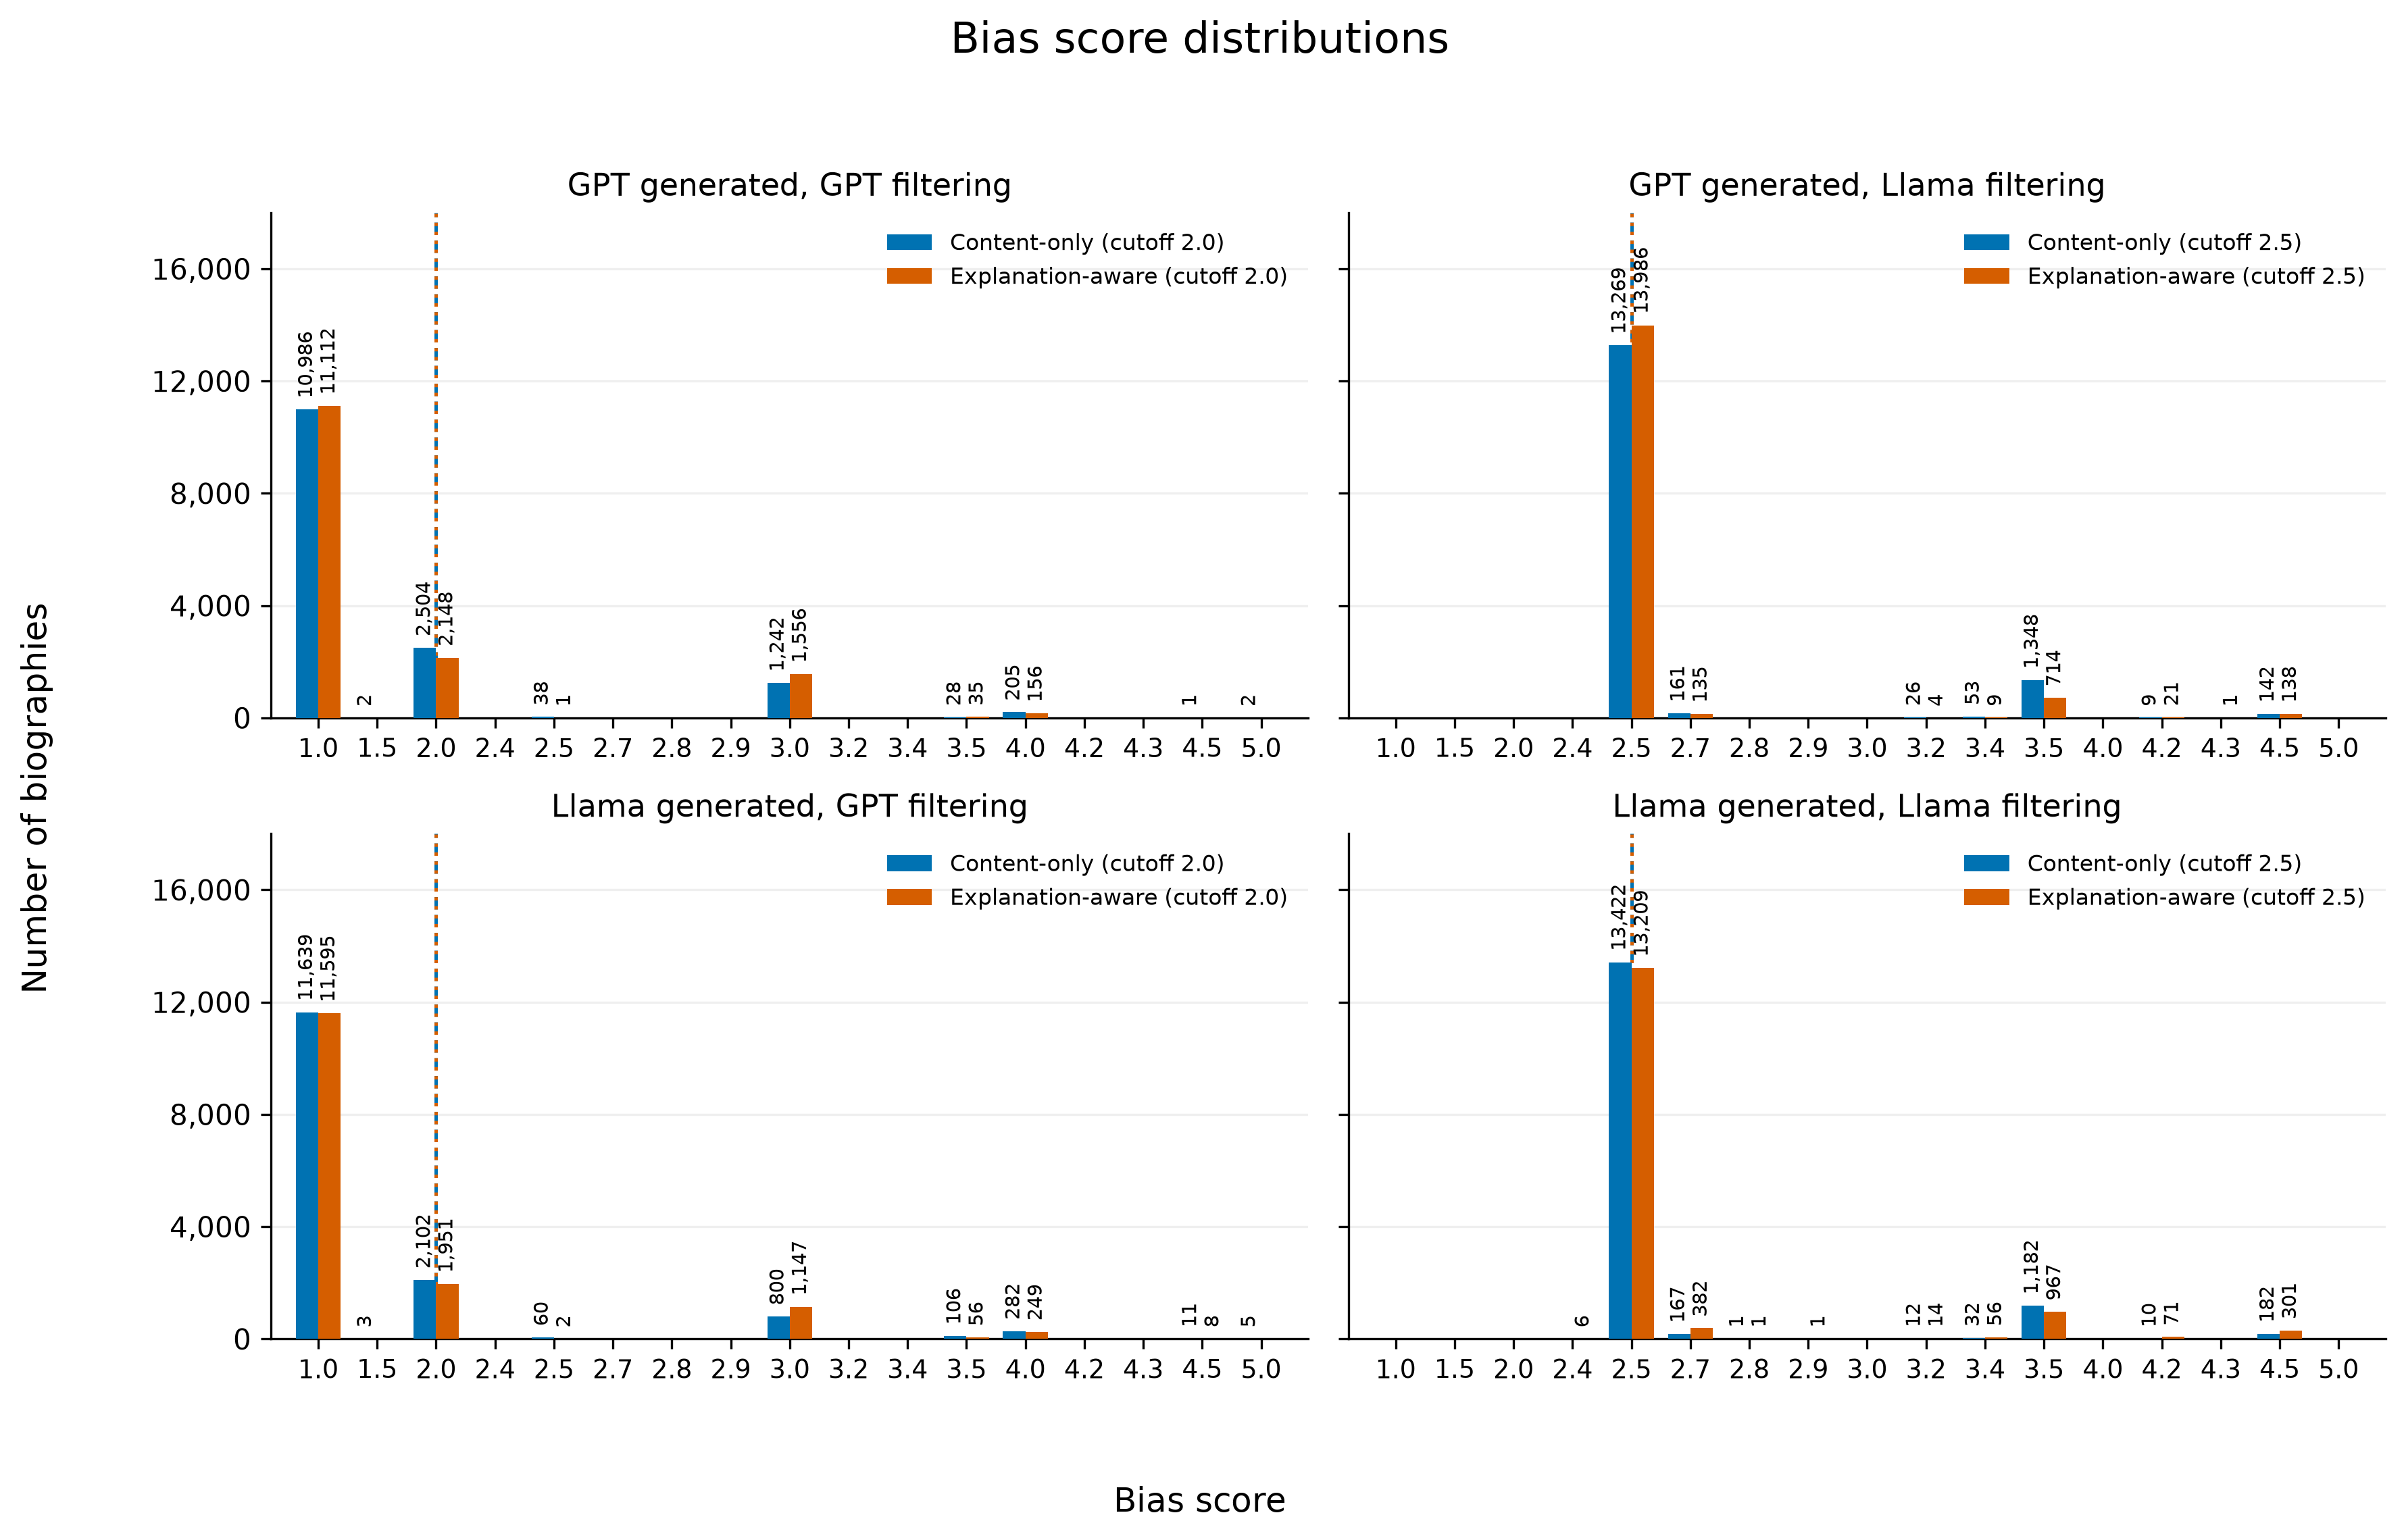
\includegraphics[width=\linewidth]{figures/filtering_score_distributions.png}
    \caption{Gender bias score distributions across all filtering configurations.}
    \Description{}
    \label{fig:filtering-scores}
\end{figure}

\begin{figure}[H]
    \centering
    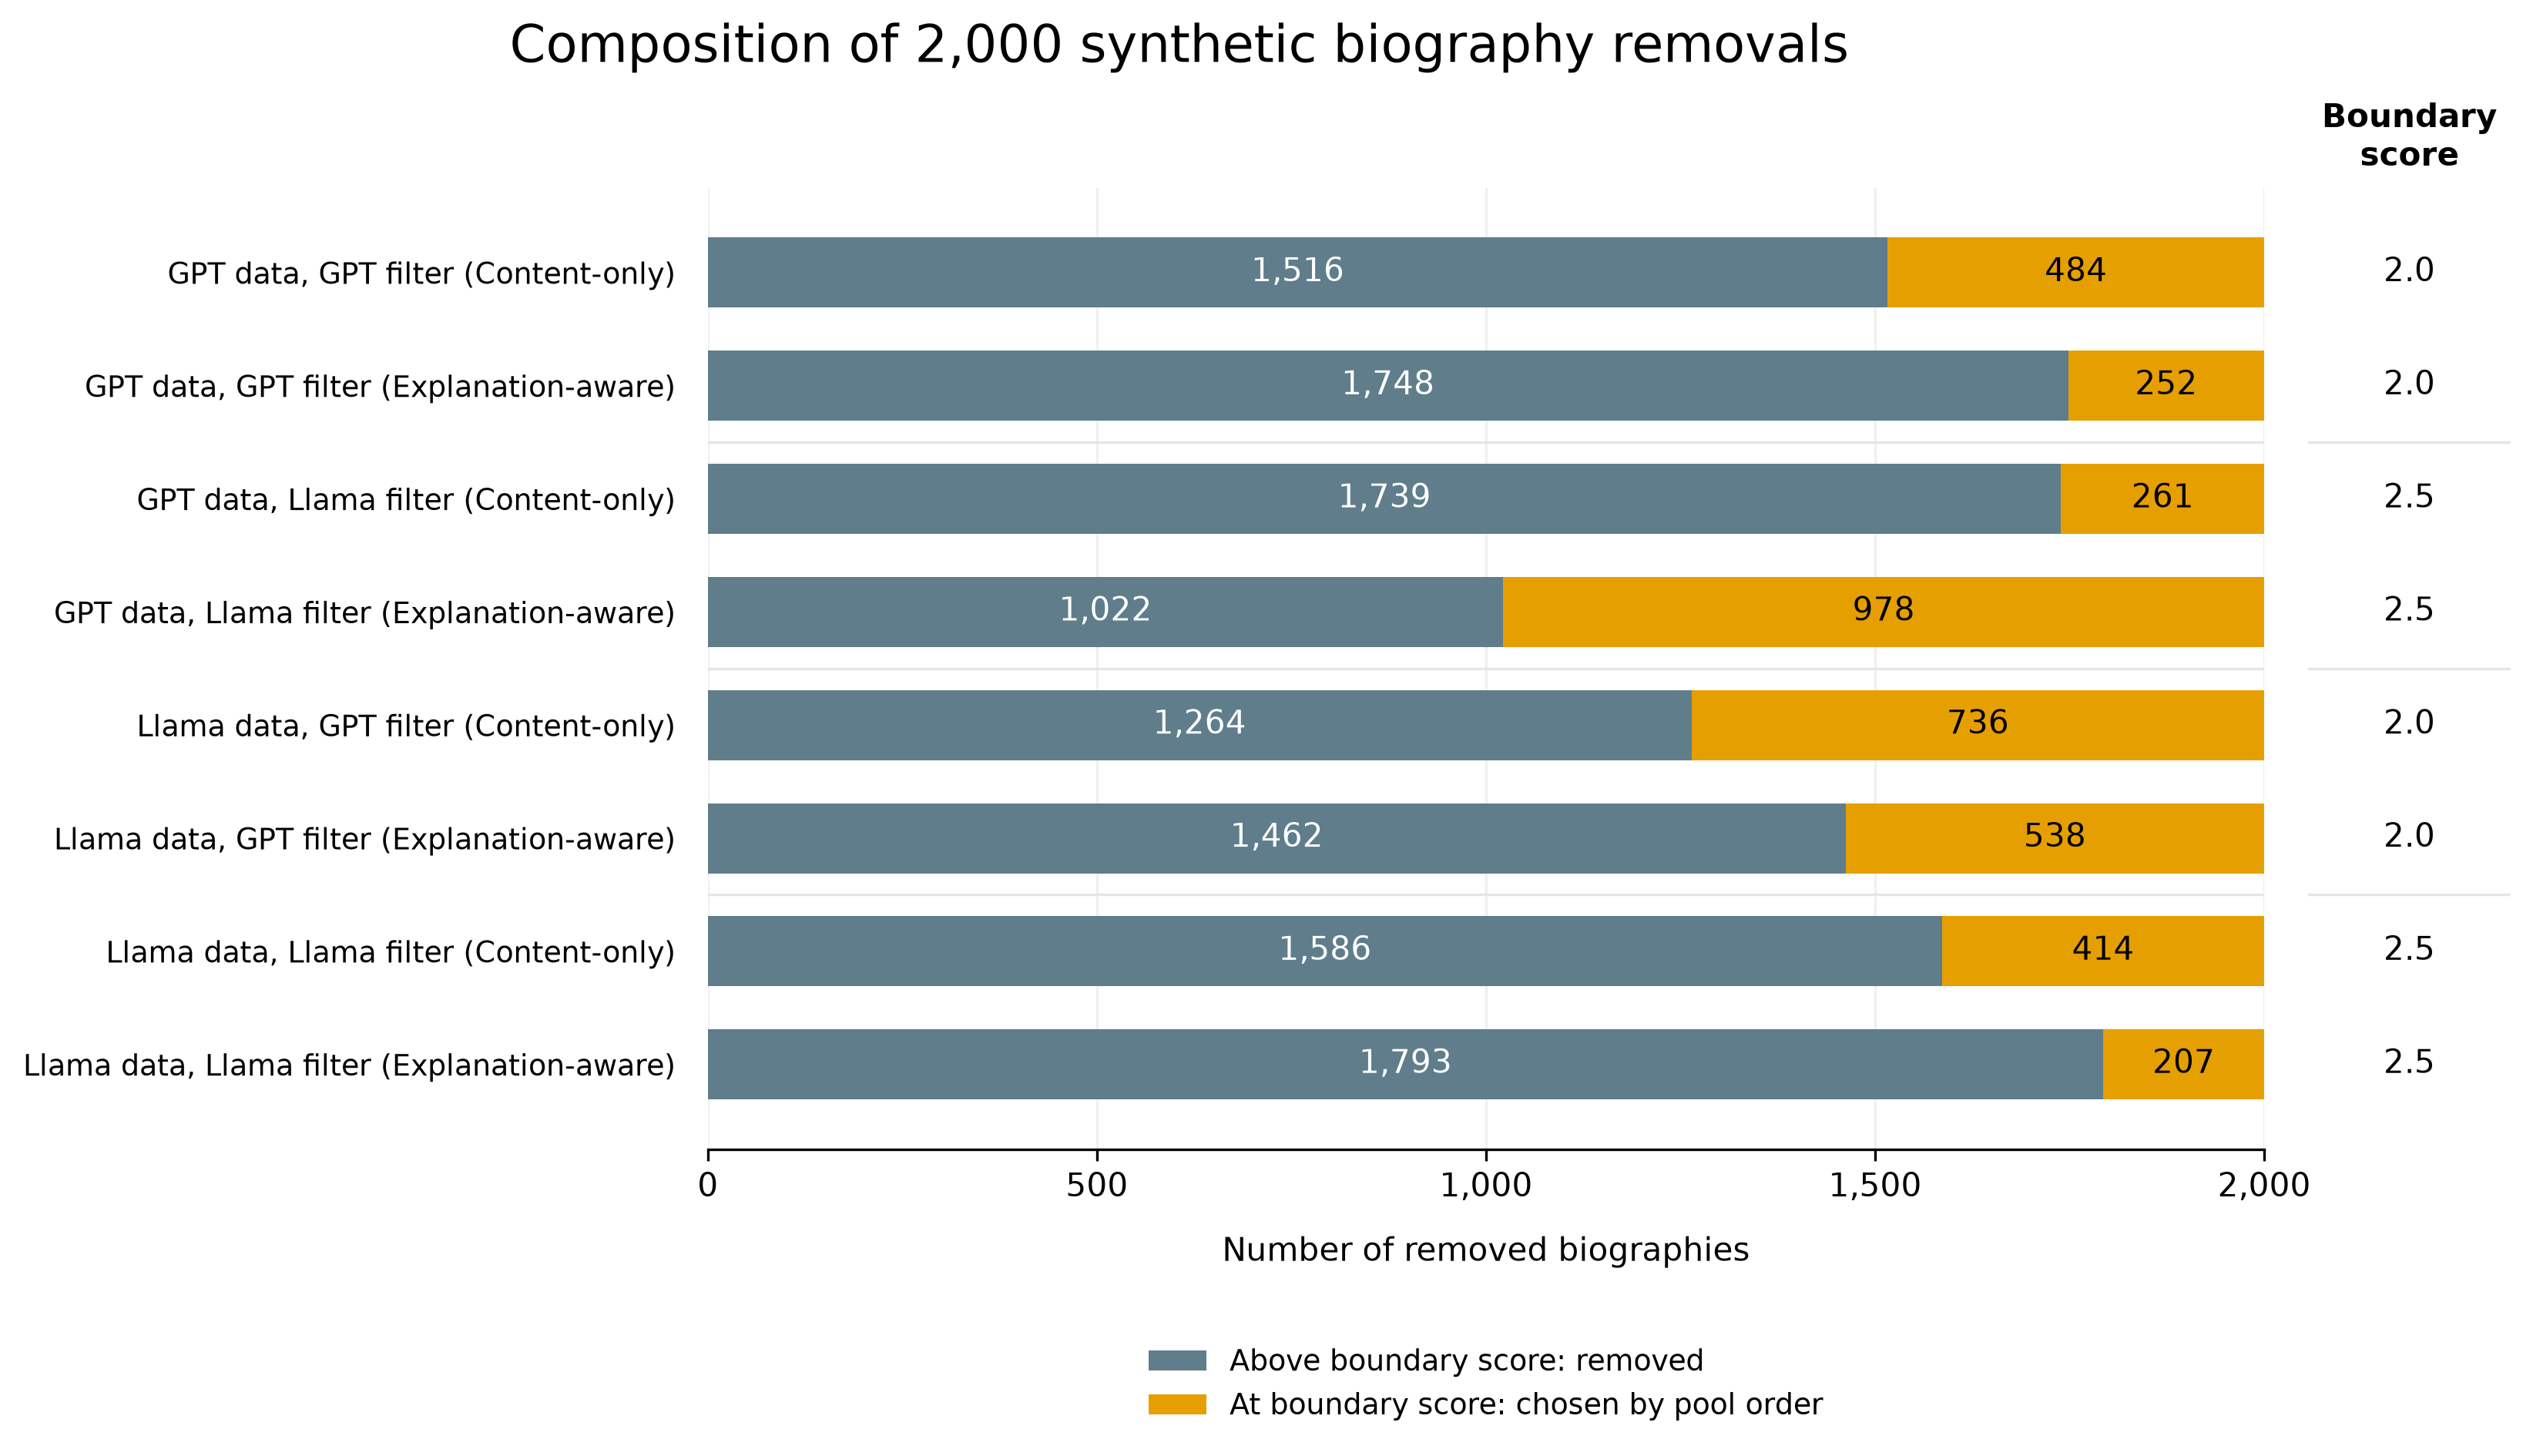
\includegraphics[width=\linewidth]{figures/filtering_removal_composition.png}
    \caption{Composition of the 2,000 biography removals across all filtering configurations.}
    \Description{}
    \label{fig:filtering-removals}
\end{figure}

\hyperref[fig:filtering-scores]{Figure~\ref*{fig:filtering-scores}} shows the distribution of the gender bias scores for all 15,008 synthetic biographies in each synthetic pool, across both generators, both scoring models and both scoring modes.
It is apparent that GPT-4o-mini gave 1.0 as the dominant score, assigned to 73.2-77.6\% of the biographies during the four runs, while for Llama-3.1-8B that was 2.5, assigned to 88.0-93.2\% of the biographies.
This difference is consistent across generator model and scoring mode.

For all configurations, the scores are concentrated at a few values, event hough all decimal scores between 1.0 and 5.0 were allowed by the few-shot prompt.
For GPT-4o-mini as scorer model, they were mostly concentrated at 1.0, 2.0, 3.0 and 4.0, while for Llama-3.1-8B that was 2.5, 2.7, 3.5 and 4.5.
The distributions were similar between scoring modes, and there was no consistent shift towards higher or lower scores.

The cutoff score is the boundary score after selecting the 2,000 highest scores. This means a fraction of the biographies with this score is removed, while the rest is kept.
For GPT-4o-mini and Llama-3.1-8B filtering the cutoff scores are 2.0 and 2.5, respectively. Both are consistent across all configurations.

\hyperref[fig:filtering-removals]{Figure~\ref*{fig:filtering-removals}} shows how the 2,000 biographies that were removed in each run were divided between biographies scoring above the cutoff value, and scoring at the cutoff value that were removed by pool order.
The number of biographies removed by pool order ranged from 207 (10.4\%) to 978 (48.9\%).
The explanation-aware scoring mode resulted in less biograhies that were removed by synthetic pool order in all configurations, except for Llama-3.1-8B filtering on GPT-4o-mini generated synthetic data.

\subsection{Downstream Classification Performance and Gender Bias}
\label{sec:downstream-results}

\hyperref[tab:downstream-all]{Table~\ref*{tab:downstream-all}} summarizes the 14 models evaluated on the same 3,998 test biographies. GPT and Llama refer to GPT-4o-mini and Llama-3.1-8B-Instruct, respectively. Macro F1 is averaged over the 28 occupations, and responses that could not be parsed are counted as errors. We summarize gender differences using the root mean square (RMS) and mean absolute (MA) TPR gaps across occupations; lower values indicate smaller disparities. Shared baselines appear only once.

\begin{table*}[t]
\centering
\small
\caption{Classification performance and gender TPR gaps. Accuracy and macro F1 are percentages; gaps are in percentage points.}
\label{tab:downstream-all}
\begin{tabular}{lllrrrrr}
\toprule
Generator & Filter & Training condition & Accuracy & Macro F1 & RMS gap & MA gap & Unparsed \\
\midrule
-- & -- & Base model & 71.21 & 73.29 & 12.60 & 8.55 & 142 \\
-- & -- & Original only & 85.29 & 84.94 & 9.72 & 7.56 & 14 \\
\midrule
GPT & -- & Full pool & 84.84 & 84.32 & 7.16 & 5.77 & 7 \\
GPT & -- & Random & 85.42 & 84.93 & 9.30 & 7.29 & 15 \\
Llama & -- & Full pool & 84.87 & 84.02 & 7.31 & 5.80 & 6 \\
Llama & -- & Random & 84.82 & 84.48 & 10.39 & 7.95 & 12 \\
\midrule
GPT & GPT & Content only & 85.12 & 85.03 & 10.81 & 8.01 & 22 \\
GPT & GPT & Explanation aware & 85.29 & 85.04 & 8.73 & 6.39 & 11 \\
GPT & Llama & Content only & 85.24 & 85.13 & 11.02 & 8.55 & 24 \\
GPT & Llama & Explanation aware & 84.87 & 84.80 & 9.59 & 7.62 & 22 \\
Llama & GPT & Content only & 85.27 & 84.87 & 10.90 & 8.18 & 9 \\
Llama & GPT & Explanation aware & 85.22 & 84.73 & 9.74 & 7.63 & 15 \\
Llama & Llama & Content only & 85.04 & 84.38 & 11.27 & 8.99 & 2 \\
Llama & Llama & Explanation aware & 83.17 & 83.53 & 14.09 & 10.22 & 25 \\
\bottomrule
\end{tabular}
\end{table*}


\begin{figure*}[!t]
    \centering
    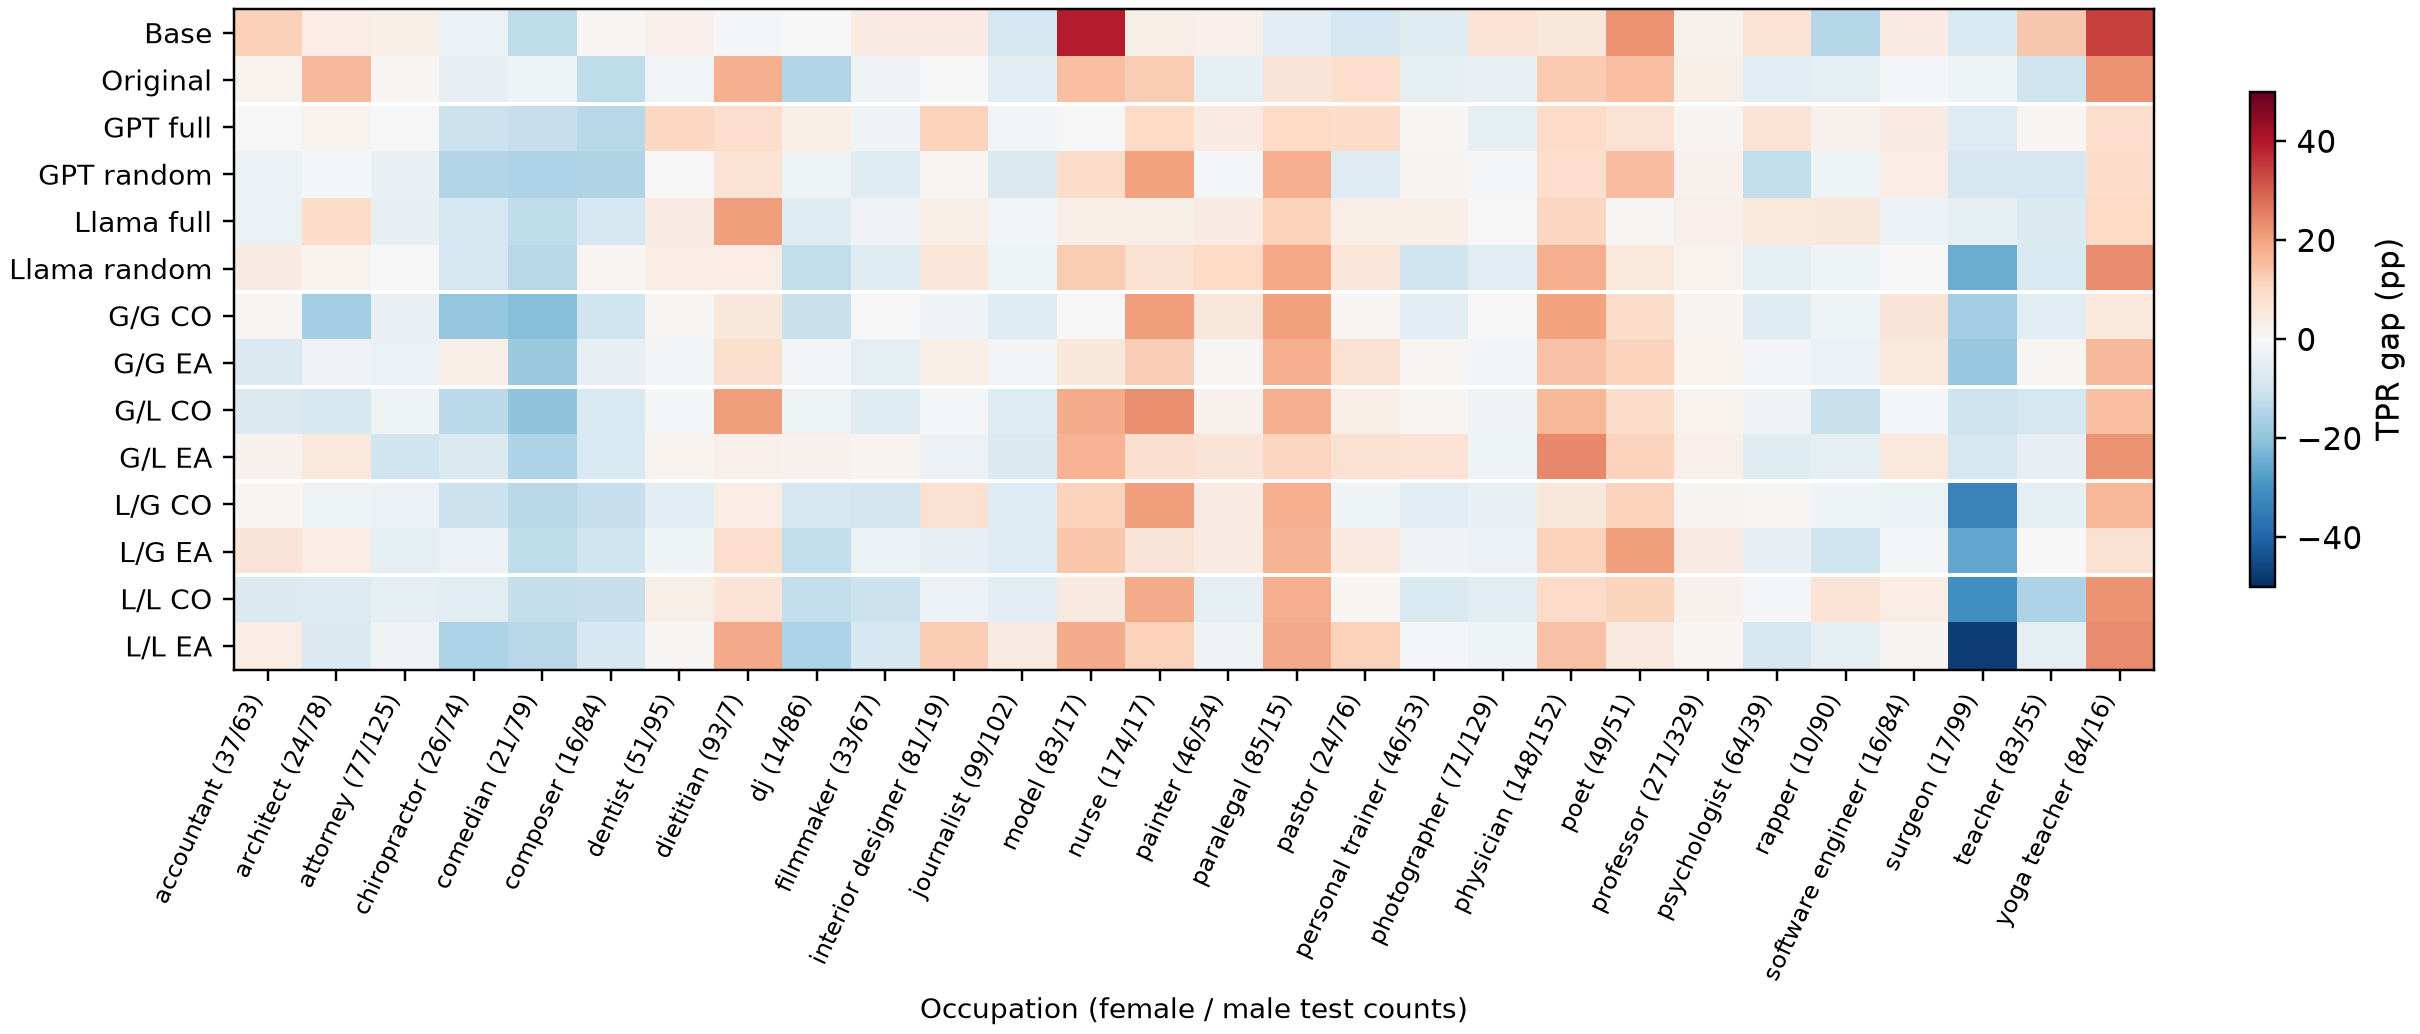
\includegraphics[width=\textwidth]{figures/downstream_tpr_gaps.png}
    \caption{TPR gender gaps by occupation, in percentage points (female minus male). G/L labels identify the generator followed by the filter; CO and EA denote content-only and explanation-aware filtering. Counts in parentheses are female/male test examples.}
    \Description{Heatmap of signed gender TPR gaps across occupations and model configurations. Red indicates higher female TPR and blue indicates higher male TPR. Each occupation is labeled with its female and male test support.}
    \label{fig:downstream-tpr-gaps}
\end{figure*}

Fine-tuning on the original data increased accuracy from 71.21\% to 85.29\% and macro F1 from 73.29\% to 84.94\%, while reducing the RMS TPR gap from 12.60 to 9.72 percentage points. Adding the full GPT or Llama pool reduced the gap further, to 7.16 and 7.31 points, but macro F1 fell slightly to 84.32\% and 84.02\%. Using all synthetic examples therefore gave smaller gender gaps at a small cost in classification performance compared with training on the original data alone.

Adding explanations reduced both RMS and MA TPR gaps in three of the four generator--filter combinations (\hyperref[tab:explanation-pairs]{Table~\ref*{tab:explanation-pairs}}). The largest RMS reduction occurred when GPT was used for both generation and filtering, with almost no change in macro F1. Using different model families for the two steps also gave smaller gaps, with slight decreases in macro F1. Llama/Llama was the exception: explanations increased the RMS gap by 2.82 percentage points and reduced macro F1 by 0.85 points.

\begin{table}[H]
\centering
\small
\setlength{\tabcolsep}{3pt}
\caption{Effect of generator explanations on macro F1 and RMS TPR gaps. CO: content only; EA: explanation aware. Differences ($\Delta$) are EA minus CO, in percentage points.}
\label{tab:explanation-pairs}
\begin{tabular}{@{}lrrrrrr@{}}
\toprule
 & \multicolumn{3}{c}{Macro F1} & \multicolumn{3}{c}{RMS TPR gap} \\
\cmidrule(lr){2-4}\cmidrule(l){5-7}
Gen./filter & CO & EA & $\Delta$ & CO & EA & $\Delta$ \\
\midrule
GPT/GPT & 85.03 & 85.04 & +0.01 & 10.81 & 8.73 & -2.08 \\
GPT/Llama & 85.13 & 84.80 & -0.33 & 11.02 & 9.59 & -1.43 \\
Llama/GPT & 84.87 & 84.73 & -0.14 & 10.90 & 9.74 & -1.16 \\
Llama/Llama & 84.38 & 83.53 & -0.85 & 11.27 & 14.09 & +2.82 \\
\bottomrule
\end{tabular}
\end{table}


Compared with random selection from the same generator, all four content-only configurations had larger RMS and MA gaps. Explanation-aware filtering gave smaller gaps than random selection for both generators when GPT was the filter, but not when Llama was the filter. Neither filtering approach gave smaller gaps than using the corresponding full synthetic pool.

The full pools contain more training examples than the filtered and random subsets. With our limited training set, keeping these extra examples may be more useful than removing examples rated as biased. Filtering may also remove useful information for recognizing occupations in both gender groups. We cannot separate the effect of data quantity from the effect of selection in these comparisons, so this is a possible explanation for the smaller gaps rather than a confirmed cause.

Using the same model family for generation and filtering offered no consistent advantage. The GPT--GPT and Llama--Llama explanation-aware conditions had the smallest and largest RMS gaps among the filtered models, respectively.

\subsection{Occupation-Level Analysis}
\label{sec:occupation-results}

\hyperref[fig:downstream-tpr-gaps]{Figure~\ref*{fig:downstream-tpr-gaps}} shows how the TPR gaps vary by occupation. Positive values mean higher TPR for female biographies, and negative values mean higher TPR for male biographies. Some groups are small: there are only seven male dietitian biographies, so one additional correct prediction changes their TPR by about 14.3 percentage points.

Adding explanations reduced the absolute gap in 15 of the 28 occupations for GPT/GPT, Llama/GPT, and Llama/Llama, and in 13 occupations for GPT/Llama (\hyperref[tab:occupation-changes]{Table~\ref*{tab:occupation-changes}}). Even though more occupations improved than worsened for Llama/Llama, its overall RMS gap increased. This is possible because RMS squares the gaps before averaging, giving more weight to large differences.

\begin{table}[!htbp]
    \centering
    \caption{Number of occupations with smaller, larger, or unchanged absolute TPR gaps after adding explanations.}
    \label{tab:occupation-changes}
    \small
    \begin{tabular}{llrrr}
        \toprule
        Generator & Filter & Smaller & Larger & Unchanged \\
        \midrule
        GPT & GPT & 15 & 13 & 0 \\
        GPT & Llama & 13 & 14 & 1 \\
        Llama & GPT & 15 & 13 & 0 \\
        Llama & Llama & 15 & 13 & 0 \\
        \bottomrule
    \end{tabular}
\end{table}

Surgeon is one example of this effect (\hyperref[tab:occupation-examples]{Table~\ref*{tab:occupation-examples}}). For Llama/Llama, adding explanations reduced female TPR from 47.1\% to 29.4\%, while male TPR changed little, from 77.8\% to 76.8\%. The absolute gap grew from 30.7 to 47.4 percentage points, contributing to the higher overall RMS gap. However, there are only 17 female surgeon biographies. The drop represents just three fewer correct predictions, from eight to five, which limits what we can conclude from it.

\begin{table}[!htbp]
    \centering
    \caption{Group-specific TPRs (\%) for selected comparisons. Configuration lists generator/filter; F and M denote female and male groups. CO: content-only; EA: explanation-aware.}
    \label{tab:occupation-examples}
    \small
    \setlength{\tabcolsep}{4pt}
    \begin{tabular}{lllrrr}
        \toprule
        Occupation & Configuration & Group & $n$ & CO & EA \\
        \midrule
        Surgeon & Llama/Llama & F & 17 & 47.1 & 29.4 \\
                &             & M & 99 & 77.8 & 76.8 \\
        \addlinespace
        Teacher & GPT/GPT & F & 83 & 60.2 & 66.3 \\
                &         & M & 55 & 65.5 & 65.5 \\
        \addlinespace
        Teacher & Llama/GPT & F & 83 & 59.0 & 56.6 \\
                &           & M & 55 & 63.6 & 56.4 \\
        \addlinespace
        Nurse & GPT/GPT & F & 174 & 91.4 & 82.8 \\
              &         & M & 17 & 70.6 & 70.6 \\
        \bottomrule
    \end{tabular}
\end{table}

A pattern that appeared in all eight filtered conditions was higher female TPR for physician, with gaps of 5.6 to 23.9 percentage points. This occupation has 148 female and 152 male test examples. Male physician biographies were also more often incorrectly classified as surgeon in every filtered condition. With GPT generation and content-only GPT filtering, for example, this happened for 37 of 152 male examples, compared with nine of 148 female examples. The models repeatedly confused these two occupations, but the predictions alone do not explain why.

For teacher, a smaller gap did not always mean better predictions. With GPT/GPT, female TPR rose from 60.2\% to 66.3\%, while male TPR stayed at 65.5\%. With Llama/GPT, however, TPR fell for both groups, reaching 56.6\% for women and 56.4\% for men. The groups became almost equal because performance declined, especially for men. A similar case occurred for nurse with GPT/GPT: the gap narrowed because female TPR fell while male TPR stayed the same.

When combining female and male test examples, no occupation had higher TPR in all four generator--filter combinations after adding explanations. Female TPR did increase in all four combinations for pastor, personal trainer, and yoga teacher, though often by only a few correct predictions. For professor, both groups improved in three of the four combinations. The gains were therefore limited to particular occupations, groups, and model combinations.

These comparisons are exploratory. Time constraints allowed only one training seed (42) per configuration, and all models were evaluated on the same test set. A pattern across several configurations is therefore not evidence from independent repetitions, and we do not claim statistical significance. Changes in occupation--gender composition after filtering and the use of pool order to break score ties could also affect the results; we did not isolate their effects.

% References are kept here so the draft remains a standalone source file.
% They can be moved to BibTeX when the remaining sections are added.
\FloatBarrier
\balance
\begin{thebibliography}{3}

\bibitem{brown2020language}
Tom B. Brown et al. 2020.
Language Models are Few-Shot Learners.
In \emph{Advances in Neural Information Processing Systems},
Vol. 33.
\url{https://arxiv.org/abs/2005.14165}

\bibitem{chen2024alpagasus}
Lichang Chen, Shiyang Li, Jun Yan, Hai Wang,
Kalpa Gunaratna, Vikas Yadav, Zheng Tang,
Vijay Srinivasan, Tianyi Zhou, Heng Huang,
and Hongxia Jin. 2024.
AlpaGasus: Training a Better Alpaca with Fewer Data.
In \emph{International Conference on Learning Representations}.
\url{https://arxiv.org/abs/2307.08701}

\bibitem{dearteaga2019bios}
Maria De-Arteaga, Alexey Romanov, Hanna Wallach, Jennifer Chayes, Christian Borgs, Alexandra Chouldechova, Sahin Geyik, Krishnaram Kenthapadi, and Adam Tauman Kalai. 2019.
Bias in Bios: A Case Study of Semantic Representation Bias in a High-Stakes Setting.
In \emph{Proceedings of the Conference on Fairness, Accountability, and Transparency}.
\url{https://arxiv.org/abs/1901.09451}

\bibitem{li2026inheritance}
Miaomiao Li, Hao Chen, Yang Wang, Tingyuan Zhu, Weijia Zhang, Kaijie Zhu, Kam-Fai Wong, and Jindong Wang. 2026.
Understanding and Mitigating Bias Inheritance in LLM-based Data Augmentation on Downstream Tasks.
\emph{arXiv preprint arXiv:2502.04419}, version 3.
\url{https://arxiv.org/abs/2502.04419v3}

\bibitem{turpin2023unfaithful}
Miles Turpin, Julian Michael, Ethan Perez, and Samuel R. Bowman. 2023.
Language Models Don't Always Say What They Think: Unfaithful Explanations in Chain-of-Thought Prompting.
In \emph{Advances in Neural Information Processing Systems}, Vol.~36.
\url{https://arxiv.org/abs/2305.04388}

\end{thebibliography}

\end{document}
